\section{Sistem Operasi}
	\subsection{Definisi}
		\begin{enumerate}
			\item Sistem operasi (OS) adalah sistem perangkat lunak yang mengelola hardware dan sumber daya perangkat lunak dengan menyediakan pelayanan secara umum untuk program komputer.

			Sistem operasi berbagi waktu menjadwalkan tugas untuk penggunaan sistem yang efisien dan mungkin juga termasuk perangkat lunak akuntansi untuk alokasi biaya waktu prosesor, penyimpanan massal, pencetakan, dan sumber daya lainnya.
			Untuk fungsi perangkat keras seperti input dan output dan alokasi memori, sistem operasi bertindak sebagai perantara antara program dan perangkat keras komputer, meskipun kode aplikasi biasanya dijalankan langsung oleh perangkat keras dan sering membuat panggilan sistem ke fungsi OS atau terganggu oleh saya t. Sistem operasi banyak ditemukan pada perangkat komputer,telepon seluler dan konsol permainan video ke server web dan superkomputer.

			\item Sistem operasi berbagi waktu menjadwalkan tugas untuk penggunaan sistem yang efisien dan mungkin juga termasuk perangkat lunak akuntansi untuk alokasi biaya waktu prosesor, penyimpanan massal, pencetakan, dan sumber daya lainnya.
			\item Untuk fungsi perangkat keras seperti input dan output dan alokasi memori, sistem operasi bertindak sebagai perantara antara program dan perangkat keras komputer, meskipun kode aplikasi biasanya dijalankan langsung oleh perangkat keras dan sering membuat panggilan sistem ke fungsi OS atau terganggu oleh saya t. Sistem operasi banyak ditemukan pada perangkat komputer,telepon seluler dan konsol permainan video ke server web dan superkomputer.

			\item Sistem operasi desktop yang dominan adalah Microsoft Windows dengan pangsa pasar sekitar 82,74%. macOS oleh Apple Inc. berada di tempat kedua (13,23%), dan varietas Linux secara kolektif berada di tempat ketiga (1,57%). Di sektor seluler (gabungan ponsel dan tablet), penggunaan pada tahun 2017 adalah hingga 70% dari Google Android dan menurut data kuartal ketiga 2016, Android pada smartphone dominan dengan 87,5 persen dan tingkat pertumbuhan 10,3 persen per tahun, diikuti oleh Apple iOS dengan 12,1 persen dan penurunan per tahun di pangsa pasar 5,2 persen, sementara jumlah sistem operasi lainnya hanya 0,3 persen. Distribusi Linux dominan di sektor server dan superkomputer. Kelas khusus lainnya dari sistem operasi, seperti embedded dan sistem real-time, ada untuk banyak aplikasi.
		\end{enumerate}
	\begin{figure}[ht]
		\centerline{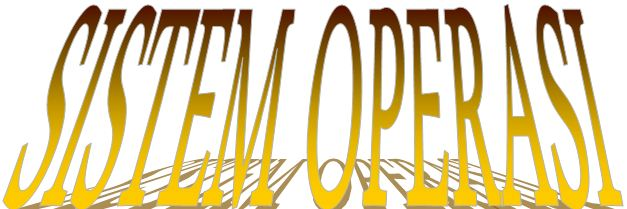
\includegraphics[width=1\textwidth]{figures/OS.JPG}}
		\caption{Sistem Operasi}
		\label{OS}
	\end{figure}

\subsection{Jenis sistem operasi}
\subsubsection{Single dan multi-tasking}
	\begin{enumerate}
		\item Sistem satu tugas hanya dapat menjalankan satu program dalam satu waktu, sementara sistem operasi multi-tasking memungkinkan lebih dari satu program berjalan dalam konkurensi. Ini dicapai dengan time-sharing, di mana waktu prosesor yang tersedia dibagi antara beberapa proses. Proses ini masing-masing terganggu berulang kali dalam irisan waktu oleh subsistem penjadwalan tugas dari sistem operasi. Multi-tasking dapat dicirikan dalam tipe preemptif dan kooperatif. Dalam preemptive multitasking, sistem operasi memotong waktu CPU dan mendedikasikan slot untuk masing-masing program. Sistem operasi mirip Unix, seperti Solaris dan Linux — serta non-Unix-like, seperti AmigaOS — mendukung multitasking preemptif. Multitasking kooperatif dicapai dengan mengandalkan pada setiap proses untuk menyediakan waktu untuk proses lain dengan cara yang ditentukan. Versi 16-bit Microsoft Windows menggunakan multi-tasking kooperatif. Versi 32-bit dari Windows NT dan Win9x, menggunakan preemptive multi-tasking.
	\end{enumerate}
\subsection{Single dan multi-user}
	\begin{enumerate}
		\item 1. Sistem operasi pengguna tunggal tidak memiliki fasilitas untuk membedakan pengguna, tetapi dapat memungkinkan beberapa program berjalan bersama-sama. Sistem operasi multi-pengguna memperluas konsep dasar multi-tasking dengan fasilitas yang mengidentifikasi proses dan sumber daya, seperti ruang disk, milik beberapa pengguna, dan sistem memungkinkan banyak pengguna untuk berinteraksi dengan sistem pada saat yang bersamaan. 
		\item 2. Sistem operasi berbagi waktu menjadwalkan tugas untuk penggunaan sistem yang efisien dan mungkin juga termasuk perangkat lunak akuntansi untuk alokasi biaya waktu prosesor, penyimpanan massal, pencetakan, dan sumber daya lainnya untuk banyak pengguna.
	\end{enumerate}
\subsection{Pendistribusian}
	\begin{enumerate}
		\item Sistem operasi terdistribusi mengelola sekelompok komputer yang berbeda dan membuatnya tampak sebagai komputer tunggal. Pengembangan jaringan komputer yang dapat dihubungkan dan berkomunikasi satu sama lain menimbulkan komputasi terdistribusi. Komputasi terdistribusi dilakukan pada lebih dari satu mesin. Ketika komputer dalam kelompok bekerja dalam kerja sama, mereka membentuk sistem terdistribusi.
	\end{enumerate}
\subsection{Sejarah}
	\begin{enumerate}
		\item Komputer awal dibangun untuk melakukan serangkaian tugas tunggal, seperti kalkulator. Fitur-fitur sistem operasi dasar dikembangkan pada tahun 1950-an, seperti fungsi monitor penduduk yang dapat secara otomatis menjalankan program yang berbeda secara berurutan untuk mempercepat pemrosesan. Sistem operasi tidak ada dalam bentuk modern dan lebih kompleks hingga awal 1960-an. Fitur perangkat keras ditambahkan, yang memungkinkan penggunaan pustaka runtime, interupsi, dan pemrosesan paralel. Ketika komputer pribadi menjadi populer pada tahun 1980-an, sistem operasi dibuat untuk mereka yang serupa dalam konsep untuk yang digunakan pada komputer yang lebih besar.

		Pada 1940-an, sistem digital elektronik paling awal tidak memiliki sistem operasi. Sistem elektronik saat ini diprogram pada deretan switch mekanis atau oleh kabel jumper pada papan steker. Ini adalah sistem tujuan khusus yang, misalnya, menghasilkan tabel balistik untuk militer atau mengontrol pencetakan cek gaji dari data pada kartu kertas berlubang. Setelah komputer tujuan umum yang dapat diprogram diciptakan, bahasa mesin (terdiri dari string digit biner 0 dan 1 pada pita kertas berlubang) diperkenalkan yang mempercepat proses pemrograman.
		\item Pada awal 1950-an, komputer hanya dapat menjalankan satu program dalam satu waktu. Setiap pengguna memiliki satu-satunya penggunaan komputer untuk jangka waktu terbatas dan akan tiba pada waktu yang dijadwalkan dengan program dan data pada kartu kertas berlubang atau pita berlubang. Program akan dimuat ke dalam mesin, dan mesin akan diatur untuk bekerja sampai program selesai atau crash. Program umumnya dapat di-debug melalui panel depan menggunakan saklar beralih dan lampu panel. Dikatakan bahwa Alan Turing adalah seorang ahli dalam mesin Manchester Mark 1 awal ini, dan dia sudah mendapatkan konsep primitif dari sistem operasi dari prinsip-prinsip mesin Turing universal.
		Kemudian mesin datang dengan perpustakaan program, yang akan dikaitkan dengan program pengguna untuk membantu dalam operasi seperti input dan output dan menghasilkan kode komputer dari kode simbolik yang dapat dibaca manusia. Ini adalah awal dari sistem operasi modern. Namun, mesin masih menjalankan pekerjaan tunggal pada suatu waktu. Di Cambridge University di Inggris, antrian pekerjaan pada suatu waktu adalah garis pencucian (garis pakaian) dari mana kaset digantung dengan pakaian warna berbeda untuk menunjukkan prioritas pekerjaan. 

		\item Pada 1940-an, sistem digital elektronik paling awal tidak memiliki sistem operasi. Sistem elektronik saat ini diprogram pada deretan switch mekanis atau oleh kabel jumper pada papan steker. Ini adalah sistem tujuan khusus yang, misalnya, menghasilkan tabel balistik untuk militer atau mengontrol pencetakan cek gaji dari data pada kartu kertas berlubang. Setelah komputer tujuan umum yang dapat diprogram diciptakan, bahasa mesin (terdiri dari string digit biner 0 dan 1 pada pita kertas berlubang) diperkenalkan yang mempercepat proses pemrograman.
		\item Pada awal 1950-an, komputer hanya dapat menjalankan satu program dalam satu waktu. Setiap pengguna memiliki satu-satunya penggunaan komputer untuk jangka waktu terbatas dan akan tiba pada waktu yang dijadwalkan dengan program dan data pada kartu kertas berlubang atau pita berlubang. Program akan dimuat ke dalam mesin, dan mesin akan diatur untuk bekerja sampai program selesai atau crash. Program umumnya dapat di-debug melalui panel depan menggunakan saklar beralih dan lampu panel. Dikatakan bahwa Alan Turing adalah seorang ahli dalam mesin Manchester Mark 1 awal ini, dan dia sudah mendapatkan konsep primitif dari sistem operasi dari prinsip-prinsip mesin Turing universal.
		\item Kemudian mesin datang dengan perpustakaan program, yang akan dikaitkan dengan program pengguna untuk membantu dalam operasi seperti input dan output dan menghasilkan kode komputer dari kode simbolik yang dapat dibaca manusia. Ini adalah awal dari sistem operasi modern. Namun, mesin masih menjalankan pekerjaan tunggal pada suatu waktu. Di Cambridge University di Inggris, antrian pekerjaan pada suatu waktu adalah garis pencucian (garis pakaian) dari mana kaset digantung dengan pakaian warna berbeda untuk menunjukkan prioritas pekerjaan. 

	\end{enumerate}
\subsection{Mikrokomputer}
	\begin{enumerate}
		\item Mikrokomputer pertama tidak memiliki kapasitas atau kebutuhan untuk sistem operasi yang rumit yang telah dikembangkan untuk mainframe dan miniis, sistem operasi minimalis dikembangkan, sering dimuat dari ROM dan dikenal sebagai monitor. Salah satu sistem operasi disk awal yang terkenal adalah CP / M, yang didukung oleh banyak mikrokomputer awal dan sangat ditiru oleh Microsoft MS-DOS, yang menjadi sangat populer sebagai sistem operasi yang dipilih untuk PC IBM . Pada 1980-an, Apple Computer Inc.  meninggalkan seri mikrokomputer Apple II yang populer untuk memperkenalkan komputer Apple Macintosh dengan antarmuka pengguna grafis inovatif  ke Mac OS.

		\item Pengenalan chip CPU Intel 80386 pada bulan Oktober 1985,  dengan arsitektur 32-bit dan kemampuan paging, menyediakan komputer pribadi dengan kemampuan untuk menjalankan sistem operasi multitasking seperti komputer minikomputer dan mainframe sebelumnya. Microsoft merespon perkembangan ini dengan mempekerjakan Dave Cutler, yang telah mengembangkan sistem operasi VMS untuk Digital Equipment Corporation. Dia dijadikan pemimpin dalam proses  pengembangan sistem operasi Windows NT, yang terus-menerus berfungsi sebagai dasar untuk jalur/way sistem operasi Microsoft. Steve Jobs, co-founder Apple Inc., memulai NeXT Computer Inc., yang mengembangkan sistem operasi NEXTSTEP. NEXTSTEP nantinya akan diakuisisi oleh Apple Inc. dan digunakan, bersama dengan kode dari FreeBSD sebagai inti dari Mac OS X.

		\item Pengenalan chip CPU Intel 80386 pada bulan Oktober 1985,  dengan arsitektur 32-bit dan kemampuan paging, menyediakan komputer pribadi dengan kemampuan untuk menjalankan sistem operasi multitasking seperti komputer minikomputer dan mainframe sebelumnya. Microsoft merespon perkembangan ini dengan mempekerjakan Dave Cutler, yang telah mengembangkan sistem operasi VMS untuk Digital Equipment Corporation. Dia dijadikan pemimpin dalam proses  pengembangan sistem operasi Windows NT, yang terus-menerus berfungsi sebagai dasar untuk jalur/way sistem operasi Microsoft. Steve Jobs, co-founder Apple Inc., memulai NeXT Computer Inc., yang mengembangkan sistem operasi NEXTSTEP. NEXTSTEP nantinya akan diakuisisi oleh Apple Inc. dan digunakan, bersama dengan kode dari FreeBSD sebagai inti dari Mac OS X.

		\item Proyek GNU dimulai oleh aktivis dan programmer Richard Stallman dengan tujuan menciptakan penggantian perangkat lunak gratis yang lengkap ke sistem operasi UNIX yang berpemilik. Meskipun proyek ini sangat berhasil dalam menduplikasi fungsionalitas berbagai bagian UNIX, pengembangan kernel GNU Hurd terbukti tidak produktif. Pada tahun 1991, mahasiswa ilmu komputer Finlandia Linus Torvalds, dengan kerja sama dari sukarelawan yang berkolaborasi melalui Internet, merilis versi pertama dari kernel Linux. Itu segera bergabung dengan komponen ruang pengguna GNU dan perangkat lunak sistem untuk membentuk sistem operasi yang lengkap. Sejak itu, kombinasi dari dua komponen utama biasanya hanya disebut Linux oleh industri perangkat lunak, konvensi penamaan yang Stallman dan Free Software Foundation tetap lawan, lebih memilih nama GNU / Linux. Berkeley Software Distribution, adalah bagian dari UNIX yang dirancang oleh University of California, Berkeley, dimulai pada thn 1970-an. Di distribusikan secara bebas dan diberikan ke banyak minikomputer, akhirnyapun mereka  memperoleh pengikut untuk digunakan pada PC, terutama sebagai FreeBSD, NetBSD dan OpenBSD.
	\end{enumerate}
\subsection{Berkeley Software Distribution}
	\begin{enumerate}
		\item Subkelompok keluarga Unix adalah keluarga Distribusi Perangkat Lunak Berkeley, yang mencakup FreeBSD, NetBSD, dan OpenBSD. Sistem operasi ini paling sering ditemukan di webservers, meskipun mereka juga dapat berfungsi sebagai OS komputer pribadi. Internet berutang banyak Kebijaksanaan untuk BSD, karena banyak dari protokol sekarang digunakan oleh komputer untuk menghubungkan, mengirim dan menerima data melalui jaringan diimplementasikan dan disempurnakan di BSD. World Wide Web Juga pertama kali dilakukan pada komputer yang menjalankan OS berdasarkan BSD yang disebut NeXTSTEP.

		\item Pada tahun 1974, University of California, Berkeley menciptakan sistem Unix awal. Seiring waktu, mahasiswa dan staf di departemen ilmu komputer telah mulai menambahkan program baru untuk menyederhanakan, seperti editor teks. Ketika Berkeley menerima komputer VAX baru pada tahun 1978 dengan Unixempat, para siswa di sekolah berbakat Unix lebih banyak menggunakan perangkat keras komputer. Departemen Pertahanan Advanced Defense Agency tertarik, dan memutuskan untuk mendanai proyek tersebut. Banyak sekolah, perusahaan, dan organisasi pemerintah menggunakan versi Berkeley dari Unix dan bukan yang resmi yang digunakan oleh AT & T.

		\item Pada tahun 1974, University of California, Berkeley menciptakan sistem Unix awal. Seiring waktu, mahasiswa dan staf di departemen ilmu komputer telah mulai menambahkan program baru untuk menyederhanakan, seperti editor teks. Ketika Berkeley menerima komputer VAX baru pada tahun 1978 dengan Unixempat, para siswa di sekolah berbakat Unix lebih banyak menggunakan perangkat keras komputer. Departemen Pertahanan Advanced Defense Agency tertarik, dan memutuskan untuk mendanai proyek tersebut. Banyak sekolah, perusahaan, dan organisasi pemerintah menggunakan versi Berkeley dari Unix dan bukan yang resmi yang digunakan oleh AT & T.

		\item Steve Jobs, setelah Apple Inc. pada tahun 1985, membentuk NeXT Inc., perusahaan yang memproduksi komputer high-end yang berjalan di bawah kondisi yang sama seperti BSD yang disebut NeXTSTEP. Salah satu komputer ini oleh Tim Berners-Lee sebagai webserver pertama yang menciptakan World Wide Web.
		\item Pengembang seperti Keith Bostic mendorong proyek untuk mengurus kode non-bebas yang berasal dari Bell Labs. Setelah ini dilakukan, bagaimanapun, AT & T menuntut. Setelah dua tahun sengketa hukum, proyek BSD menghasilkan beberapa derivatif gratis, seperti NetBSD dan FreeBSD (keduanya pada tahun 1993), dan OpenBSD (dari NetBSD pada tahun 1995).
	\end{enumerate}
\subsection{Linux}
	\begin{enumerate}
		\item Kernel Linux berasal pada tahun 1991, sebagai proyek Linus Torvalds, sementara seorang mahasiswa di Finlandia. Dia memposting informasi tentang proyek-proyek di newsgroup untuk siswa komputer dan programer, dan Menerima dan membantu dari sukarelawan yang berhasil membuat kernel yang lengkap dan fungsional. Linux adalah Unix-like, tetapi dikembangkan tanpa kode Unix, tidak seperti BSD dan variannya. Karena model lisensi terbuka, kode kernel Linux tersedia untuk studi dan modifikasi, yang digunakan pada berbagai mesin dari superkomputer ke jam tangan pintar. Meskipun mereka menggunakan Linux pada 1,82% dari semua PC "desktop" (atau laptop), itu umumnya telah diadopsi untuk server embedded dan sistem seperti ponsel. Linux telah menemukan Unix pada banyak platform dan juga pada kebanyakan superkomputer termasuk 385 teratas. Banyak dari komputer yang sama juga menggunakan Green500 (tetapi dalam urutan yang berbeda), dan Linux berjalan di atas 10. Linux juga dapat digunakan pada perangkat kecil lainnya. komputer hemat energi, seperti smartphone dan jam pintar. Linux kernel dalam beberapa distribusi populer, seperti Red Hat, Debian, Ubuntu, Linux Mint dan Google Android, Chrome OS, dan Chromium OS.
	\end{enumerate}
\subsection{macOS}
	\begin{enumerate}
		\item macOS (sebelumnya Mac OS X dan kemudian OS X) juga merupakan sistem operasi grafis inti yang dikembangkan, dipasarkan dan dijual oleh Apple Inc., yang terbaru yang telah dimuat sebelumnya pada semua komputer Macintosh yang sedang dikirimkan. MacOS adalah penerus asli dari Mac OS klasik, yang telah menjadi sistem operasi utama Apple sejak 1984. Tidak seperti pendahulunya, ia telah dikembangkan di NeXT hingga tahun 1980-an dan sampai Apple membeli perusahaan tersebut awal tahun 1997. Mac OS X Server 1.0, diikuti pada Maret 2001 oleh versi klien (Mac OS X v10.0 Cheetah). Sejak itu, enam klien dan edisi server yang lebih baik dari mac OS telah dirilis, untuk hal yang sama di OS X 10.7 Lion. Sebelum bergabung dengan macOS, edisi server - MacOS Server - adalah sama seperti mitra desktop dan juga berjalan di lini perangkat Apple Macintosh. MacOS Server menyertakan manajemen grup dan perangkat lunak yang mencakup akses ke layanan jaringan utama, termasuk transfer surat, server Samba, server LDAP, server nama domain, dan banyak lagi. Dengan Mac OS X v10.7 Lion, semua aspek server Mac OS X Server telah diintegrasikan ke dalam versi klien dan produk tersebut bermerek kembali sebagai OS X (menjatuhkan "Mac" dari namanya). Alat server sekarang tersedia sebagai aplikasi.
	\end{enumerate}
\subsection{Microsoft Windows}
	\begin{enumerate}
		\item Microsoft Windows adalah sistem operasi yang dirancang oleh Microsoft Corporation dan khususnya untuk komputer arsitektur Intel, dengan dimensi 88,9 persen dari total pada komputer yang terhubung dengan Web. Versi terbaru adalah Windows 10.

		 \item Pada 2011, Windows 7 mengambil alih Windows XP sebagai versi yang sangat umum. Microsoft Windows pertama kali dirilis pada tahun 1985, yang merupakan bagian dari MS-DOS, yang merupakan sistem operasi yang digunakan pada saat itu. Pada tahun 1995, Windows 95 dirilis hanya menggunakan MS-DOS sebagai bootstrap. Untuk menyelesaikan retret, Win9x dapat menjalankan driver MS-DOS dan Windows-3 Windows 16-bit yang nyata. Windows ME, dirilis pada tahun 2000, adalah versi terbaru dalam keluarga Win9x. Versi yang lebih baru sekarang didasarkan pada kernel Windows NT. Tanggung jawab Windows saat ini berjalan pada mikroprosesor ARM IA-32, x86-64, dan 32-bit. Selain itu Itanium masih didukung pada server lama versi Windows Server 2008 R2. Di masa lalu, Windows NT mendukung arsitektur tambahan. Server edisi Windows banyak digunakan. 
		\item Dalam beberapa tahun terakhir, Microsoft telah mengeluarkan modal yang signifikan dalam upayanya ke Windows sebagai sistem operasi server. Namun, penggunaan Windows pada server tidak meluas seperti pada komputer pribadi karena Windows bersaing dengan Linux dan BSD untuk server pasar. ReactOS adalah sistem operasi Windows alternatif, yang sedang dikembangkan pada prinsip-prinsip Windows - tanpa menggunakan kode Microsoft.

		\item Pada 2011, Windows 7 mengambil alih Windows XP sebagai versi yang sangat umum. Microsoft Windows pertama kali dirilis pada tahun 1985, yang merupakan bagian dari MS-DOS, yang merupakan sistem operasi yang digunakan pada saat itu. Pada tahun 1995, Windows 95 dirilis hanya menggunakan MS-DOS sebagai bootstrap. Untuk menyelesaikan retret, Win9x dapat menjalankan driver MS-DOS dan Windows-3 Windows 16-bit yang nyata. Windows ME, dirilis pada tahun 2000, adalah versi terbaru dalam keluarga Win9x. Versi yang lebih baru sekarang didasarkan pada kernel Windows NT. Tanggung jawab Windows saat ini berjalan pada mikroprosesor ARM IA-32, x86-64, dan 32-bit. Selain itu Itanium masih didukung pada server lama versi Windows Server 2008 R2. Di masa lalu, Windows NT mendukung arsitektur tambahan. Server edisi Windows banyak digunakan. Dalam beberapa tahun terakhir, Microsoft telah mengeluarkan modal yang signifikan dalam upayanya ke Windows sebagai sistem operasi server. Namun, penggunaan Windows pada server tidak meluas seperti pada komputer pribadi karena Windows bersaing dengan Linux dan BSD untuk server pasar. ReactOS adalah sistem operasi Windows alternatif, yang sedang dikembangkan pada prinsip-prinsip Windows - tanpa menggunakan kode Microsoft.

	\end{enumerate}
	
	
\cite{silberschatz2014operating}
\cite{hoare1974monitors}
\cite{bach1986design}
\cite{love2005linux}
\cite{kukreja2006rui}
\cite{mckeown2009software}
\cite{russinovich2005microsoft}
\cite{van1994treecon}
\cite{mckusick1985performance}
\cite{higgins1988clustal}
